\documentclass[11pt,a4paper]{article}

\usepackage{epsfig}
\usepackage{multicol}

\usepackage[utf8]{inputenc}
\usepackage[brazil]{babel}
\usepackage{fancyheadings}
\usepackage{amsmath}
\usepackage{calrsfs}
\usepackage{enumerate}
\usepackage{enumitem}   
\DeclareGraphicsExtensions{.png,.pdf}
\usepackage{amsmath, amsfonts, amssymb}
\usepackage{esint}
\usepackage{graphicx}
\usepackage{multicol}
\usepackage{tasks}
\usepackage[utf8]{inputenc}
\usepackage{mathrsfs} % Transformada de Laplace
\usepackage{indentfirst}
\usepackage{xcolor}

% As margens
\setlength{\textheight}{24.0cm}
\setlength{\textwidth}{17.5cm}
\setlength{\oddsidemargin}{2.0cm} % Margens reais desejadas
\setlength{\evensidemargin}{2.0cm} % 2+17.5+1.5=21cm (largura A4)
\setlength{\topmargin}{1.5cm} % 1.5+1.6+1.0+24.0+1.6=29.7cm
\setlength{\headheight}{1.6cm} % (altura A4)
\setlength{\headsep}{1.0cm}
\setlength{\columnsep}{1.5cm} % Coluna = 8cm ((17.5-1.5)/2)
\addtolength{\oddsidemargin}{-1in}
\addtolength{\evensidemargin}{-1in}
\addtolength{\topmargin}{-1in}
\setlength{\footskip}{0.0cm}


% Novos comandos
\newcommand{\limite}{\displaystyle\lim}
\newcommand{\integral}{\displaystyle\int}
\newcommand{\somatorio}{\displaystyle\sum}
\newcommand{\mat}[1]{\mbox{\boldmath{$#1$}}} 

\pagestyle{fancy}


\usepackage{lipsum}

\lhead{

\includegraphics[width=1cm]{brasao.png}
}

\rhead{ 
\sc\textbf{U}niversidade \textbf{F}ederal do \textbf{C}eará\\
Campus Quixadá\\ Lista 1 de Eletromagnetismo}

\cfoot{}

\begin{document}

	\begin{center}
		\Large Eletrostática - Lei de Coulomb. 
	\end{center}

\begin{flushleft}
\textbf{Nome:} Mateus Sousa Araújo. \\
\textbf{Matrícula:} 374858. \\
\textbf{Professor:} Antônio Joel Ramiro de Castro. \\
\textbf{Curso:} Engenharia de Computação. \\
\end{flushleft}

\begin{enumerate}

\item \textbf{Griffiths - Cap. 2 - Problema 2.2.}

\begin{figure}[h]	
\centering % para centralizarmos a figura	
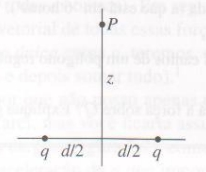
\includegraphics[width=4cm]{Selection_070.jpg} 
\caption{Cargas separadas a uma distância $d$.}
\end{figure}

\begin{enumerate}
\item Encontre o campo elétrico (magnitude, direção e sentido) a uma distância $z$ acima do ponto central entre duas cargas iguais, $q$, que estão separadas por uma distância $d$. Verifique se o resultado é coerente com o que se espera quando $z >> d$.

\textbf{RESOLUÇÃO}

Primeiramente, é preciso verificar a atuação dos campos elétricos gerados pelas duas cargas no ponto P. 

\begin{figure}[h]	
\centering % para centralizarmos a figura	
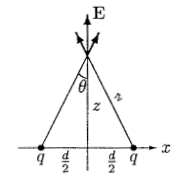
\includegraphics[width=4cm]{Selection_073.jpg} 
\caption{Campos elétricos gerados pelas duas cargas no ponto P.}
\end{figure}

Pode-se perceber que, pela decomposição de forças, as componentes horizontais se cancelam. Apenas duas componentes no eixo vertical se somarão, e dessa forma podemos descobrir o campo resultante $E_z$ neste ponto . Dessa forma, podemos escrever:


\begin{center}

$\vec{E_z} = 2 E\cos \theta$.

$\vec{E_z} = \displaystyle\dfrac{1}{4 \pi \epsilon_0} \displaystyle\dfrac{2q}{r^2}\cos \theta $.

$r^2 = z^2 + \left(\displaystyle\dfrac{d}{2}\right)^2$.

\end{center}

Substituindo $\cos \theta$ e o valor de $r$ temos:

\begin{center}
$\vec{E} = \displaystyle\dfrac{1}{4 \pi \epsilon_0} \displaystyle\dfrac{2qz}{\left(z^2 + \left(\displaystyle\dfrac{d}{2}\right)^2\right)^{3/2}}$.
\end{center}

Quando $z >> d$, temos que a contribuição de campo no ponto P é dado pela soma das duas cargas, ou seja, $2q$. Logo, o campo elétrico na direção $z$ fica:

\begin{center}
$\vec{E} = \displaystyle\dfrac{1}{4 \pi \epsilon_0} \displaystyle\dfrac{2q}{\left(z^2\right)}$.
\end{center}

\item Repita a parte (a), só que desta vez faça a carga do lado direito igual a $-q$ em vez de $+q$.

\textbf{RESOLUÇÃO}

Quando a carga da direita assume sinal negativo, temos que o campo resultante no ponto P atuará de forma diferente como foi visto no item $a$. Dessa vez, as componentes na direção vertical se cancelam, resultando apenas a soma das componentes na direção $x$.

\begin{figure}[h]	
\centering % para centralizarmos a figura	
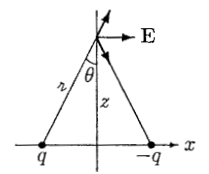
\includegraphics[width=4cm]{Selection_074.jpg} 
\caption{Atuação do campo resultante no ponto P após a carga da direita ficar com sinal negativo.}
\end{figure}

Dessa forma, podemos escrever:

\begin{center}
$\vec{E_z} = \displaystyle\dfrac{1}{4 \pi \epsilon_0} \displaystyle\dfrac{2q}{r^2}\sin \theta $.
\end{center}

Assim como no item a, podemos substituir os valores de $\sin \theta$ e o valor de $r$. Dessa forma, temos:

\begin{center}
$\vec{E} = \displaystyle\dfrac{1}{4 \pi \epsilon_0} \displaystyle\dfrac{qd}{\left(z^2 + \left(\displaystyle\dfrac{d}{2}\right)^2\right)^{3/2}}$.
\end{center}

Se fizermos $z >> d$, o campo elétrico na direção $\hat{x}$ se torna:

\begin{center}

$\vec{E} = \displaystyle\dfrac{1}{4 \pi \epsilon_0} \displaystyle\dfrac{qd}{\left(z^3\right)}$.

\end{center}

\end{enumerate}

\item \textbf{Griffiths - Cap. 2 - Problema 2.3.}

\begin{figure}[h]	
\centering % para centralizarmos a figura	
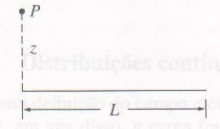
\includegraphics[width=4cm]{Selection_071.jpg} 
\caption{Segmento linear de cargas.}
\end{figure}

Encontre o campo elétrico a uma distância $z$ acima de uma das extremidades de um segmento de linha reta $L$ e que tem uma distribuição linear de carga uniforme, de densidade $\lambda$. Verifique se a sua fórmula é coerente com o que seria de se esperar para o caso de $z >> L$.

\begin{figure}[h]	
\centering % para centralizarmos a figura	
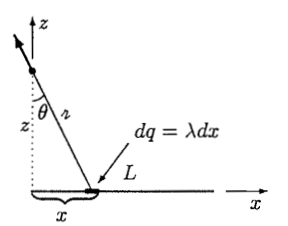
\includegraphics[width=4cm]{Selection_075.jpg} 
\caption{Campo resultante na contribuição de uma carga infinitesimal.}
\end{figure}

\textbf{RESOLUÇÃO}

É preciso saber a contribuição de campo de um elemento infinitesimal de carga ao longo de toda linha e depois intregar num intervalo de $0$ a $L$. O Campo resultante terá duas componentes em $\hat{z}$ e $\hat{x}$. É preciso calcular cada uma dessas componentes.

\begin{center}

$\vec{E_z} = \displaystyle\dfrac{1}{4 \pi \epsilon_0} \displaystyle\int_0^L\displaystyle\dfrac{\lambda \ dx}{r^2}\cos \theta \ \hat{z}$.

\end{center}

Substituindo os valores de $r$ e $\cos \theta$, temos:

\begin{center}

$\vec{E_z} = \displaystyle\dfrac{1}{4 \pi \epsilon_0} \lambda z \displaystyle\int_0^L \displaystyle\dfrac{1}{\left(x^2 + z^2\right)^{3/2}} \ dx$.

\end{center}

Essa integral basta escolher $z = x \tan \theta$ e fazer uma substituição trigonométrica. No final, retornando para a variável em $x$, temos nossa função em $z$ aplicado de $0$ a $L$:

\begin{center}

$\vec{E_z} = \displaystyle\dfrac{1}{z^2} \left[\displaystyle\dfrac{x}{\sqrt{z^2 + x^2}}\right]_0^L$.

\end{center}

No final, temos:

\begin{center}

$\vec{E_z} = \displaystyle\dfrac{1}{z^2} \left[\displaystyle\dfrac{L}{\sqrt{x^2 + L^2}}\right]$.

\end{center}


Da mesma forma, para a direção $\hat{x}$, temos:

\begin{center}

$\vec{E_x} = - \displaystyle\dfrac{1}{4 \pi \epsilon_0} \displaystyle\int_0^L\displaystyle\dfrac{\lambda \ dx}{r^2}\sin \theta \ \hat{x}$.

\end{center}

Substituindo os valores de $r$ e $\sin \theta$ na função, obtemos:

\begin{center}

$\vec{E_x} = - \displaystyle\dfrac{1}{4 \pi \epsilon_0} \lambda \displaystyle\int_0^L \displaystyle\dfrac{x}{\left(x^2 + z^2\right)^{3/2}} \ dx$.

\end{center}

Basta fazer uma susbtituição simples e aplicando os limites de integração podemos encontrar o campo na direção $\hat{x}$.

\begin{center}

$\vec{E_x} = - \displaystyle\dfrac{1}{4 \pi \epsilon_0} \lambda \left[\displaystyle\dfrac{1}{z} - \displaystyle\dfrac{1}{\sqrt{z^2 + L^2}}\right]$.

\end{center}

Agora basta juntar as duas componentes do campo resultante. 

\begin{center}

$\vec{E_x} = \displaystyle\dfrac{1}{4 \pi \epsilon_0} \displaystyle\dfrac{\lambda}{z} \left[\left(-1 + \displaystyle\dfrac{z}{\sqrt{z^2 + L^2}}\right) \hat{x} + \left(\displaystyle\dfrac{L}{\sqrt{z^2 + L^2}}\right)\hat{z}\right]$.

\end{center}

\item \textbf{Griffiths - Cap. 2 - Problema 2.6.}

\begin{figure}[h]	
\centering % para centralizarmos a figura	
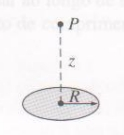
\includegraphics[width=3cm]{Selection_072.jpg} 
\caption{Disco circular plano de densidade superficial $\sigma$.}
\end{figure}

Encontre o campo elétrico a uma distância $z$ acima de um disco circular plano de raio $R$, que tem uma densidade superficial de carga uniforme $\sigma$. O que a sua fórmula revela no limite $R \to \infty$? 

\textbf{RESOLUÇÃO}

A ideia é dividir o disco em anéis concêntricos elementares e calcular o campo elétrico no ponto P somando, ou seja, integrando as contribuições de todos os anéis. O campo elétrico resultante gerado por um anel é dado por: 

\begin{center}
$\vec{dE} = \displaystyle\dfrac{1}{4 \pi \epsilon_0} \displaystyle\dfrac{dq \ z}{(z^2 + r^2)^{3/2}}$.
\end{center}

\begin{figure}[h]	
\centering % para centralizarmos a figura	
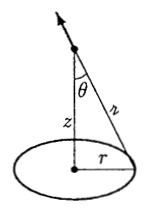
\includegraphics[width=3cm]{Selection_076.jpg} 
\caption{Carga infinitesimal gerando campo elétrico em um anel.}
\end{figure}

A área infinitesimal de um anel, é dado por $2\pi r dr$, onde $dr$ é a largura infinitesimal do mesmo. Como temos vários anéis se somando, temos uma densidade superficial de cargas. Dessa forma, podemos escrever:

\begin{center}

$dq = \sigma \ dA$.

$dq = 2 \sigma \pi r dr$.

\end{center}

Podemos substituir a relação acima em $dq$ no anel e fazer uma integração de $0$ a $R$.  

\begin{center}
$\vec{E} = \displaystyle\dfrac{1}{4 \pi \epsilon_0} 2\pi \sigma z \displaystyle\int_0^R\displaystyle\dfrac{r}{(r^2 + z^2)^{3/2}} \ dr$.
\end{center}

Após uma substituição simples, temos:

\begin{center}
$\vec{E} = \displaystyle\dfrac{1}{4 \pi \epsilon_0} 2\pi \sigma z \left[\displaystyle\dfrac{1}{z} - \displaystyle\dfrac{1}{\sqrt{R^2 + z^2}}\right] \hat{z}$.
\end{center}

Para $R \to \infty$, temos:

\begin{center}
$\vec{E} = \displaystyle\dfrac{\sigma}{2 \pi \epsilon_0} \hat{z}$.
\end{center}

\end{enumerate}
	
\end{document}